\section{Verwandte Arbeiten} \label{sec:VerwandteArbeiten}
In diesem Abschnitt werden verwandte Arbeiten vorgestellt, die auch das Layoutproblem betrachten.
Außerdem will ich auch konkrete Tools anschauen, die Metriken visualisieren und deren Ansätze betrachten.

\subsection{layouts}

So etwas ähnliches auch sagen:
A number of other hierarchy visualization techniques have been
developed [18, 23, 29, 32], including space-filling visualizations
like step trees [6], Voronoi treemaps [2] and generalized treemaps
[34]. Although relevant to hierarchy visualization, we pursue
contributions that are sufficiently distinct from such work that we
do not dwell on extensive comparisons. \cite{lu2008cascaded}

\subsubsection{Treemap layouts}
Es gibt bisher noch zu wenige ARbeiten, die sich mit dieser Frage beschäftigen. (Oder eigentlich gibt es nur eine die wirklich in die richtung geht - mehr dann bei verwandte arbeiten)


\cite{lu2008cascaded}:
Hao Lü and James Fogarty stellten in ihrem Paper \textit{Cascaded Treemaps:
Examining the Visibility and Stability of Structure in Treemaps}\cite{lu2008cascaded} fest: \enquote{an important limitation of treemaps is
the difficulty of discerning the structure of a hierarchy}\cite[1]{lu2008cascaded} Das stellt im Grunde das Problem von Treemaps dar, welches auch algorithmisch nicht einfach gelöst werden kann (siehe Abschnitt \ref{sec:TreemapProblem}). Die Idee ist anders als bei Nested Ansätzen die Kindknoten nicht einfach in den Elternknoten zu zeichnen, sondern sie leicht versetzt \textit{über} dem Elternknoten zu zeichnen (siehe Abbildung \ref{fig:cascaded}). Dadurch soll weniger Platz verloren gehen und es entsteht ein leichter 3D-Effekt.

\begin{figure}
    \centering
    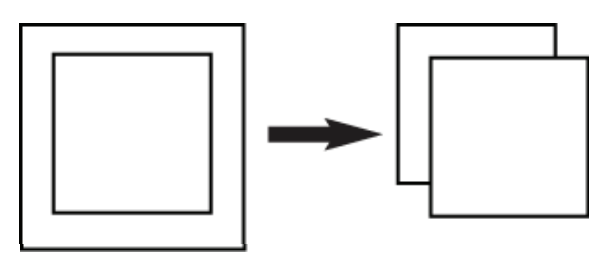
\includegraphics[width=0.8\textwidth]{images/cascaded.png}
    \caption{Links beispielhaf der Nested treemaps Ansatz, bei dem der Kindknoten einfach in dem Elternknoten gezeichnet wird. Rechts der Cascaded Treemap Ansatz, bei dem der Kindknoten als rechteck leicht versetzt nach rechts unten \textit{über} dem Elternknoten gezeichnet wird. Abbildung aus \cite[3]{lu2008cascaded}.}
    \label{fig:cascaded}
\end{figure}

Sie stellen in ihrem Paper auch fest, dass manche Knoten verschwinden können, da der Platz der für Beschriftung und abstände benötigt wird, beim Layoutschritt nicht berücksichtigt werden kann. Sie stellen einen Zwei Schrittigen ansatz vor, der im ersten schritt mit den squarify algorithmus \cite{bruls2000squarified} das layout erstellt. Im zweiten Schritt wird dann die Größe, aber nicht die Platzierung der Knoten angepasst, indem der Abstand und platz für Beschriftung berücksichtigt wird. Das Problem von verschwindenden Knoten wird dadurch nicht komplett gelöst, aber Knoten verschwinden nur noch, wenn der Platz für die Beschriftung und den Abstand größer ist als der zur Verfügung stehende Platz. 
In dem Paper wird leider nicht auf das Problem eingegangen, welches wir in Abschnitt \ref{sec:TreemapProblem} betrachtet haben, dass die Fläche, die durch Abstände eingenommen wird nicht exakt berechnet werden kann. Außerdem wird nicht beleuchtet, wie sehr sich die relation von Knotengröße und Knotenwert ändert. In diesem Paper werden wir auf beide Probleme in der tiefe eingehen und die Auswirkungen auf die darstellung untersuchen.


Die Autoren des ursprungs squarify Algorithmus \cite{bruls2000squarified} stellen in einem anderen Paper \cite{cushionTreemaps} eine Idee vor, um Struktur ohne Änderung des Layouts darzustellen undzwar mit Schatten (siehe Abbildung \ref{fig:cushion}). Dabei bekommt jeder Knoten, egal ob Eltern- oder Kindknoten, einen Innenrenschatten, wodurch die Struktur der Knoten sichbar wird.

\begin{figure}
    \centering
    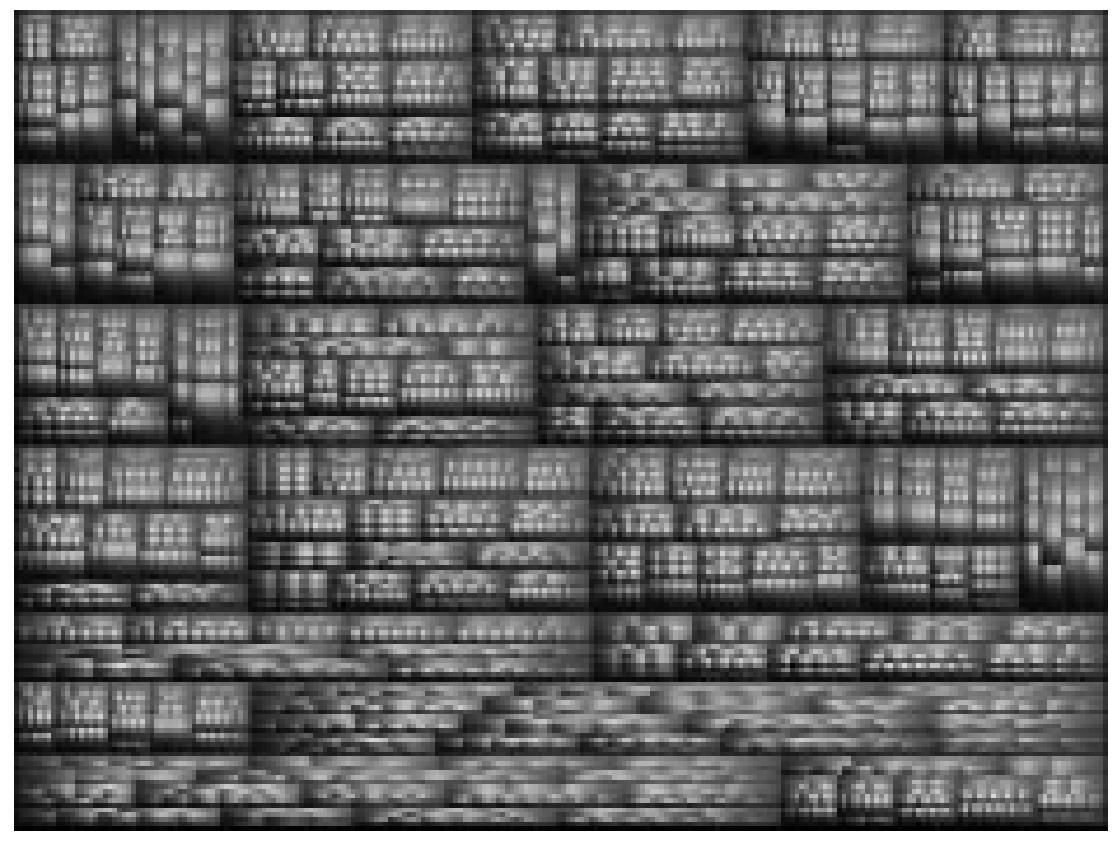
\includegraphics[width=0.8\textwidth]{images/cushionTreemap.png}
    \caption{Beispiel für eine Cushion Treemap \cite[4]{cushionTreemaps}}
    \label{fig:cushion}
\end{figure}

Peter Demian und Renate Fruchter stellen die Idee vor dass dickere outlines he höher der Knoten ist auch die Struktur verdeutlichen können. 

Nicholas Kong et al schlagen vor verschiedene Umriss dicken zu nutzen um die Struktur der Knoten darzustellen.\cite{2010-perception-treemaps} (siehe Abbildung \ref{fig:thickOutline}).

% \begin{figure}
%     \centering
%     \includegraphics[width=0.8\textwidth]{images/thickOutline.png}
%     \caption{Beispiel für eine Treemap mit verschieden dicken outlines, die die Struktur verdeutlichen sollen. Abbildung aus \cite[1]{2010-perception-treemaps}}
%     \label{fig:thickOutline}
% \end{figure}

Scheibel et al. stellen in ihrem Paper \textit{Survey of treemap layout algorithms}\cite{scheibel2020survey} eine Übersicht über die verschiedenen Treemap Layout Algorithmen vor. Sie unterscheiden zwischen den verschiedenen Ansätzen. 

Sie kategorieren die verschiedenen Ansätze in 4 Kategorien: Art der Aufteilung, zusätzliche Attribute, Layout Form und Referenzraum Dimension. 
Uns interresiert hier besonders das zusätzliche Attribut der "Werte" und die Dimension 2D (wie in Abschnitt \ref{sec:Problemstellung} beschrieben).
Arten der Aufteilung sind: Packing und splitting. Packing ist dabei die Idee, die Knoten so zu packen, dass sie möglichst wenig Platz verbrauchen und splitting ist die Idee Knoten in kleinere Knoten zu unterteilen. Alle in den Grundlagen (Abschnit \ref{sec:Treemap}) vorgestellten Algorithmen sind also splitting Algorithmen.
Sie stellen vier Layout Formen vor: Kreisförmig, rechteckig, konvex und nicht konvex. Alle in den Grundlagen vorgestellten Algorithmen sind rechteckige Layouts.
Von den untersuchten 81 Algorithmen sind 54 rechteckige Layouts und 58 splitting Algorithmen. Der in dieser ARbeit speziell untersuchte Treemap Algorithmus passt also genau in die Kategorie der meist verwendeten Ansätze.

\smallskip

\subsection{Was suchen wir} 
